\chapter{Implementation}
\label{ch:implementation}

\section{Overview}
This chapter presents the concrete implementation of DriveXR's principal subsystems, illustrated with screenshots of the running application and representative code excerpts. Where Chapter~\ref{ch:methodology} describes the development process and the decisions made, this chapter documents what was actually built, module by module.

\section{Vehicle Physics Implementation}

The player vehicle is a Tata Safari model driven by four Unity WheelCollider components configured for front-wheel drive. Figure~\ref{fig:cockpit_view} shows the in-VR cockpit view, including the steering wheel, dashboard instrumentation, and the environment visible through the windscreen.

\begin{figure}[H]
    \centering
    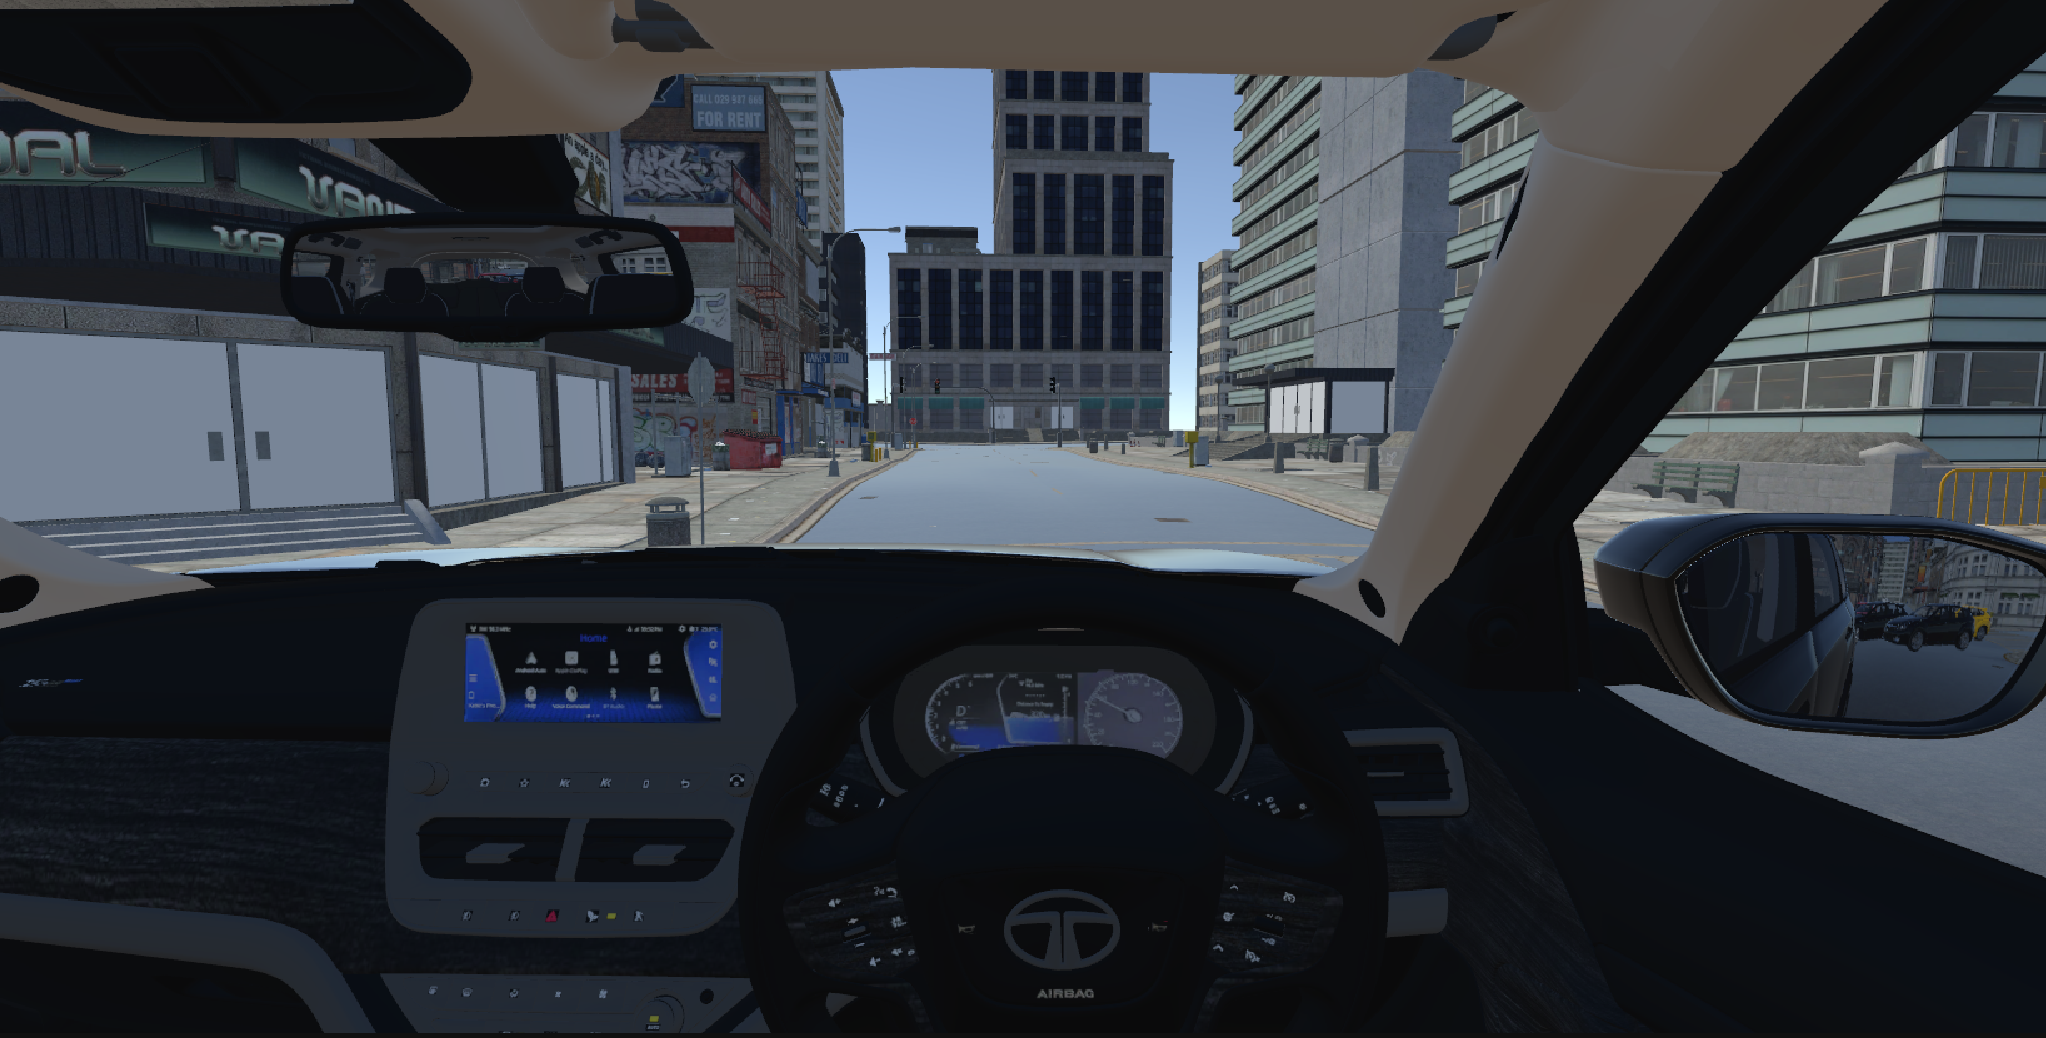
\includegraphics[width=0.8\textwidth]{figs/cockpit_view.png}
    \caption{In-VR cockpit view from the driver's seat, showing the steering wheel, dashboard, and city environment.}
    \label{fig:cockpit_view}
\end{figure}

Suspension parameters were tuned iteratively rather than derived analytically, since the priority was qualitative handling feel rather than strict physical accuracy:

\begin{verbatim}
void SetupSuspension(WheelCollider wc)
{
    JointSpring spring = wc.suspensionSpring;
    spring.spring = springStrength;
    spring.damper = springDamper;
    spring.targetPosition = 0.5f;
    wc.suspensionSpring = spring;
    wc.suspensionDistance = suspensionDistance;
    ...
}
\end{verbatim}

The gearbox is a four-position automatic (Park, Reverse, Neutral, Drive). Gear changes to Park or Reverse are rejected above a configurable speed threshold, matching real vehicle behaviour and preventing unrealistic drivetrain damage in simulation.

\section{Hardware Input Implementation}

\subsection{Racing Wheel and Pedals}
The Logitech G29 connects to the host PC via USB and is read through Unity's legacy Input System. A defining implementation challenge was the G29's pedal axis convention: the pedals report $+1$ at rest and $-1$ at full travel, the reverse of the conventional 0-to-1 range expected by most vehicle controller implementations. This was corrected with the remapping:

\begin{verbatim}
brakeInput    = Mathf.Clamp01((-rawAccel + 1f) / 2f);
throttleInput = Mathf.Clamp01((-rawBrake  + 1f) / 2f);
\end{verbatim}

\subsection{Gear Shifter}
The Logitech Driving Force Shifter presented a more significant implementation challenge than the wheel itself. Its gear gate signals were not reliably exposed through Unity's legacy Input Manager as either buttons or axes on this system configuration. This was resolved using the third-party Unity-Inputter package, which wraps the Logitech G HID SDK directly and exposes each gear gate as an indexable button state:

\begin{verbatim}
bool forward =
    g[LogitechG29.G29Button.Shifter1].isPressed ||
    g[LogitechG29.G29Button.Shifter2].isPressed ||
    g[LogitechG29.G29Button.Shifter3].isPressed ||
    ...
\end{verbatim}

Since DriveXR simulates a single-gear automatic transmission rather than a full manual gearbox, all forward gate positions on the physical H-pattern shifter map onto a single Drive gear, while one gate is mapped to Reverse. This preserves the tactile experience of a full-size shifter without requiring a manual-transmission simulation model.

% TODO: insert screenshot of the physical shifter hardware or a close-up
% of it in use, if available
% \begin{figure}[H]
%     \centering
%     \includegraphics[width=0.7\textwidth]{figs/shifter_hardware.png}
%     \caption{Logitech Driving Force Shifter used for gear selection.}
%     \label{fig:shifter_hardware}
% \end{figure}

\section{VR and XR Interaction Implementation}

\subsection{Steering Wheel Hand Interaction}
The in-VR steering wheel uses a passive interaction component (Unity's XRSimpleInteractable) rather than a physics-based grab interactable. This design choice followed a specific implementation problem encountered early in development: using a grab-type interactor caused the XR runtime to reposition the wheel mesh's transform directly, which combined with the mesh's off-centre pivot point caused the wheel to orbit around the vehicle rather than rotate in place when grabbed. The corrected implementation instead calculates a normalised steering value from the hand's angular position relative to the wheel centre, leaving the mesh's own transform hierarchy untouched by the XR interaction system.

\subsection{VR Environment Selection Menu}
A world-space UI menu, built entirely in code rather than via the Unity UI designer, allows environment selection via both hand-ray pointing and direct hand-tracking touch interaction. The menu is anchored close to the user's viewpoint by design, ensuring it is always readable and reachable regardless of where the player is looking when it is opened; as a result it is intentionally too close to the camera to be captured whole in a single screenshot, and is instead described here structurally. The menu presents three cards, one per training environment, each showing the environment's name and a short description (e.g. ``Beginner — get used to the controls'' for the straight highway). Selecting a card triggers the teleport sequence described below.

Selecting an environment triggers a teleport operation that resets the vehicle's Rigidbody velocity and angular velocity to zero before repositioning it, preventing any carry-over momentum from the previous environment:

\begin{verbatim}
rb.linearVelocity  = Vector3.zero;
rb.angularVelocity = Vector3.zero;
playerCar.transform.SetPositionAndRotation(target.position, target.rotation);
\end{verbatim}

\section{NPC Traffic System Implementation}

The NPC traffic controller was implemented as an explicit finite state machine after an earlier per-checkpoint raycast implementation proved unreliable (Chapter~\ref{ch:methodology}). Figure~\ref{fig:city_traffic} shows the city environment with multiple AI vehicles navigating a signalised intersection.

\begin{figure}[H]
    \centering
    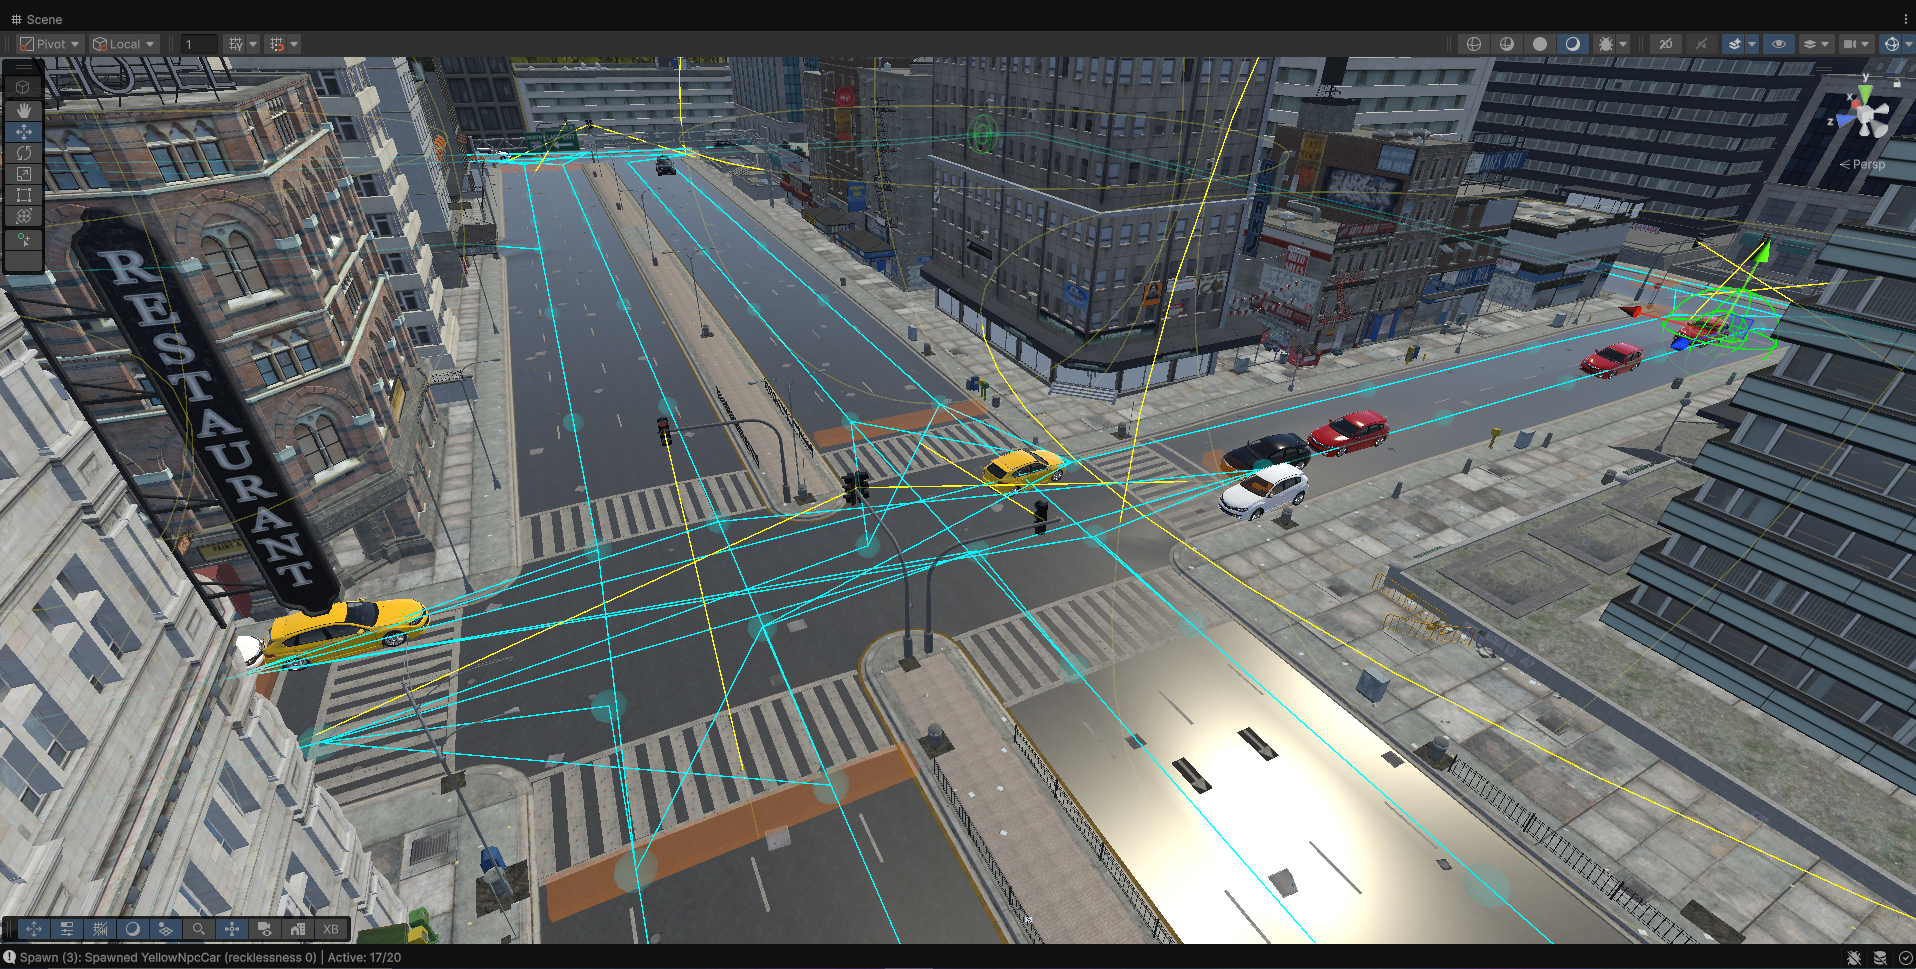
\includegraphics[width=0.8\textwidth]{figs/city_traffic.png}
    \caption{City environment showing NPC vehicles navigating a signalised intersection.}
    \label{fig:city_traffic}
\end{figure}

Obstacle detection uses a single forward sphere-cast originating from the vehicle's own centre, avoiding the sensor-offset issues present in the earlier implementation:

\begin{verbatim}
if (!Physics.SphereCast(origin, sensorRadius, transform.forward,
                        out RaycastHit hit, senseDist, seenLayers,
                        QueryTriggerInteraction.Ignore))
    return float.MaxValue;
\end{verbatim}

A watchdog recovery mechanism snaps a vehicle back onto its path if it becomes stuck on geometry or blocked in traffic beyond a configurable timeout, ensuring that individual vehicle failures do not produce permanent gridlock:

\begin{verbatim}
if (tryingToMove && kmh < 2)
{
    stuckTimer += Time.fixedDeltaTime;
    if (stuckTimer >= stuckRecoverTime)
        Recover("stuck without progress");
}
\end{verbatim}

\section{Rear-View Mirror Implementation}

Side and rear-view mirrors are implemented using dedicated off-screen cameras rendering into RenderTexture assets displayed on the mirror glass material. Each mirror camera is disabled by default and enabled for a single frame via a timed coroutine at 20 frames per second, reducing GPU overhead relative to continuous rendering. The mirrors are visible in the cockpit view already shown in Figure~\ref{fig:cockpit_view}, displaying the environment behind and to the sides of the vehicle in real time.

\section{Environment Implementation}

All three training environments coexist within a single Unity scene with spatially separated road networks, allowing instant switching without a scene reload. Figure~\ref{fig:three_environments} shows a top-down Scene view screenshot of the complete layout, with the straight highway, curved road, and city grid all visible.

\begin{figure}[H]
    \centering
    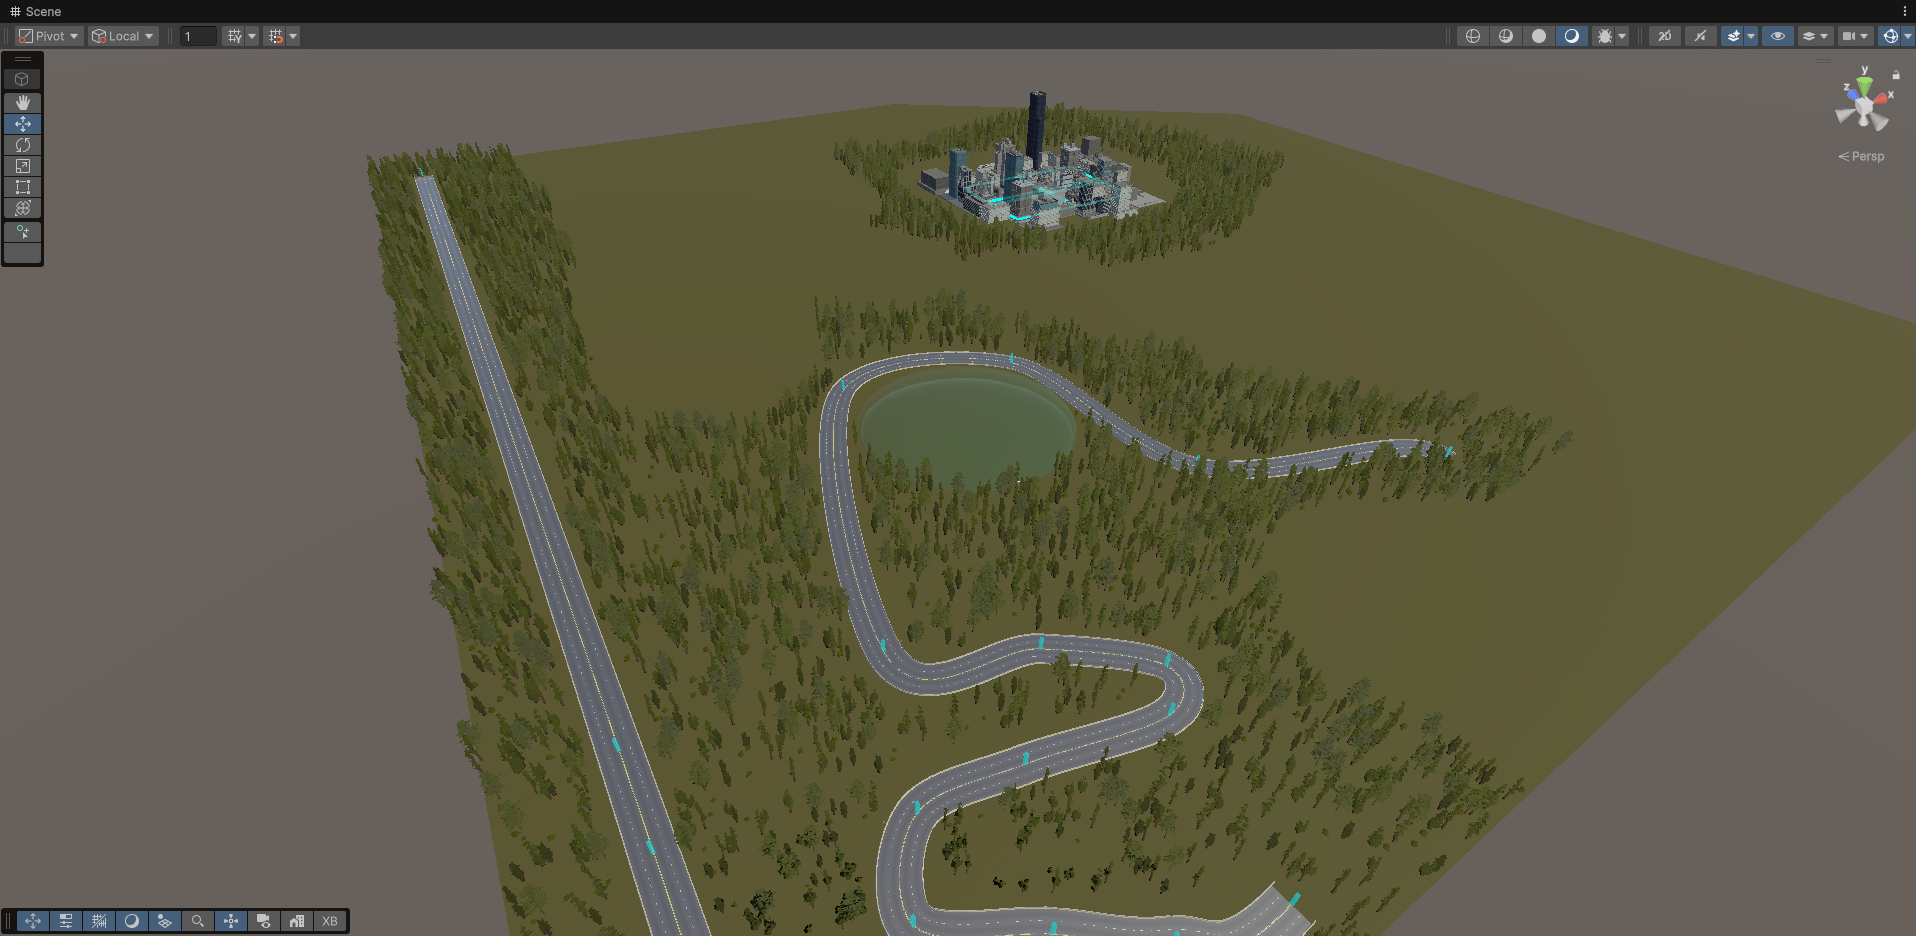
\includegraphics[width=0.9\textwidth]{figs/three_environments.png}
    \caption{Top-down Scene view showing the complete layout of the three training environments within the single DriveXR scene: straight highway, curved road, and city grid.}
    \label{fig:three_environments}
\end{figure}

\section{Summary}
This chapter has documented the concrete implementation of DriveXR's vehicle physics, hardware input, VR interaction, NPC traffic, mirror rendering, and environment systems, with reference to the specific implementation challenges encountered and resolved during development. Chapter~\ref{ch:results} presents the evaluation of these implemented systems.